\documentclass[10pt,a4paper]{article}

\usepackage{graphicx}    
\usepackage{float}
\usepackage{hyperref}                   % collegamenti ipertestuali
\usepackage[utf8]{inputenc}
\usepackage[english]{babel}
\usepackage[babel]{csquotes}
\usepackage{url}
\usepackage{graphicx}
\usepackage{lastpage}
\usepackage{fancyhdr}
\usepackage[top=1cm,bottom=4cm,left=80pt,right=80pt]{geometry} %disegna la linea
\usepackage{listings} %per grandi porzioni di codice
\usepackage{booktabs,tabularx}
\usepackage{makeidx}
\usepackage{fixltx2e}
\usepackage{hyperref}
\usepackage{enumitem}
\usepackage{color}
\usepackage[T1]{fontenc}
\usepackage{svg}
\usepackage{amsmath}
\usepackage[toc]{glossaries}
\usepackage{dirtree}
\usepackage{listings}
\usepackage{siunitx}
\usepackage[official]{eurosym}
\usepackage[export]{adjustbox}
\usepackage{calc}
\usepackage{rotating}
\usepackage{soul}
\usepackage{amsmath}

\pagestyle{fancy}
\setlength{\headheight}{2cm} %settato grandezza header

\renewcommand{\footrulewidth}{0.5pt} %ridefinisco il valore della riga di intestazione
\renewcommand{\headrulewidth}{0.5pt} %ridefinisco il valore della riga di pie' di pagina
\addtolength{\headwidth}{\marginparsep}
\addtolength{\headwidth}{\marginparwidth}

\fancyhead{} %annulla head di default
\fancyfoot{} %annulla foot di default


\newcommand{\complex}[1]{\textit{\color{blue} {#1}}}
\newcommand{\change}[1]{\textit{ \color{red}** {#1}}}

%%%%%%%%%%%%%%%%%%%%%%%%%%%%%%%%%%%%%%%%%%%%%%%%%%%%%%%%%%%%%%%%%%%%%
%    DOCUMENT TITLE

\newcommand{\doctitle}{\textbf{CondorcetFuse} \\
	 Condoret voting for run fusion}

%%%%%%%%%%%%%%%%%%%%%%%%%%%%%%%%%%%%%%%%%%%%%%%%%%%%%%%%%%%%%%%%%%%%%
%%%%%%%%%%%%%%%%%%%%%%%%%%%%%%%%%%%%%%%%%%%%%%%%%%%%%%%%%%%%%%%%%%%%%
%%%%%%%%%%%%%%%%%%%%%%%%%%%%%%%%%%%%%%%%%%%%%%%%%%%%%%%%%%%%%%%%%%%%%
%   DOCUMENT SUBTITILE
\newcommand{\docsubtitle}{Evalutation and comparison of an implementation with other fusion strategies}
%%%%%%%%%%%%%%%%%%%%%%%%%%%%%%%%%%%%%%%%%%%%%%%%%%%%%%%%%%%%%%%%%%%%%
%%%%%%%%%%%%%%%%%%%%%%%%%%%%%%%%%%%%%%%%%%%%%%%%%%%%%%%%%%%%%%%%%%%%%
%%%%%%%%%%%%%%%%%%%%%%%%%%%%%%%%%%%%%%%%%%%%%%%%%%%%%%%%%%%%%%%%%%%%%
%   DOCUMENT FOOTER 
% If not modified, footer is equal to document subtitle
\newcommand{\projectfooter}{\docsubtitle}
%%%%%%%%%%%%%%%%%%%%%%%%%%%%%%%%%%%%%%%%%%%%%%%%%%%%%%%%%%%%%%%%%%%%%
%%%%%%%%%%%%%%%%%%%%%%%%%%%%%%%%%%%%%%%%%%%%%%%%%%%%%%%%%%%%%%%%%%%%%
%%%%%%%%%%%%%%%%%%%%%%%%%%%%%%%%%%%%%%%%%%%%%%%%%%%%%%%%%%%%%%%%%%%%%


%	Logo intestazione
%\rhead{\includegraphics[scale=0.15]{}}

%	footer
\cfoot{
	\projectfooter\\
	{\doctitle}\\
}
\rfoot{
	\thepage\ di \pageref{LastPage}
}


%**************************************************************
% Impostazioni di hyperref
%**************************************************************
\hypersetup{
	%hyperfootnotes=false,
	%pdfpagelabels,
	%draft,	% = elimina tutti i link (utile per stampe in bianco e nero)
	colorlinks=true,
	linktocpage=true,
	pdfstartpage=1,
	pdfstartview=FitV,
	% decommenta la riga seguente per avere link in nero (per esempio per la stampa in bianco e nero)
	%colorlinks=false, linktocpage=false, pdfborder={0 0 0}, pdfstartpage=1, pdfstartview=FitV,
	breaklinks=true,
	pdfpagemode=UseNone,
	pageanchor=true,
	pdfpagemode=UseOutlines,
	plainpages=false,
	bookmarksnumbered,
	bookmarksopen=true,
	bookmarksopenlevel=1,
	hypertexnames=true,
	pdfhighlight=/O
}
\newcommand{\printTitle}{	
	\begin{titlepage}
		\begin{center}
			
		%	\begin{figure}[h!]	\vspace{5cm}
		%		\centering
		%		\includegraphics[width=0.7\linewidth]{}
		%	\end{figure}
			\vspace{0.3cm}
			\hrule
			\vspace{0.3cm}	
			\begin{Huge}
				\doctitle  \\			
			\end{Huge}
			\vspace{0.3cm}
			\begin{Large}
				\docsubtitle
			\end{Large}
			\vspace{0.3cm}
			
		\end{center}
		
\end{titlepage}}






\begin{document}
    \printTitle
    \newpage
    \tableofcontents
    \newpage
    %\listoftables
    %\listoffigures

    \section{Introduction}
    
    In Information Retrieval, data fusion is the combination of the results
    of independent searches on a document collection into one single output
    result set.
    
    It has been shown in the past that this can greatly improve retrieval
    effectiveness over that of the individual results.
    
    The aim of this work is to show a possible implementation of some basic
    fusion strategies and compare them to anadvanced one: Condorcet fusion \cite{3}.

    In this project the input documents were taken from the TREC TIPSTER Collection using 50 topics (topics 351-400).
    
    We organized our work as follows:

    \begin{itemize}
        \item \textbf{Indexing:} we created four different indexes:
        \begin{itemize}
        	\item Without both stemmer and stop list;
        	\item only using the Porter stemmer;
        	\item only using the stop list;
        	\item using both the Porter stemmer and the stop list;
        \end{itemize}
        \item \textbf{Retrieval:} 10 different retrieval models listed in Table \ref{tab:10Mod};
		\item \textbf{Normalization:} min/max normalization as presented by Lee \cite{1}
        \item \textbf{Fusion strategy:} we compared seven different fusion strategies:
            \begin{itemize}
                \item 6 basic strategies proposed by Fox and Shawn \cite{2} and listed in Table \ref{tab:6Fus};
                \item Condorcet fusion (advanced strategy) as proposed by Montague and Aslam \cite{3}
            \end{itemize}
    \end{itemize}

	\begin{table} [H]
		\begin{minipage} {0.3\linewidth}
			\centering
			\begin{tabular}{c}
				\toprule
				\textbf{Retrieval models} \\ \toprule
				BB2 \\
				BM25 \\
				DLH13 \\
				Hiemstra\_LM \\
				IFB2 \\
				TF\_IDF \\
				DFIC \\
				DFIZ \\
				DirichletLM \\
				InL2 \\
				\bottomrule
			\end{tabular}
			\caption{Retrieval models used}
			\label{tab:10Mod}
		\end{minipage}		
		\begin{minipage} {0.7\linewidth}
			\centering
			\begin{tabular}{c p{4cm}}
				\toprule
				\textbf{Basic fusion methods} & \textbf{New score} \\ \toprule
				CombMNZ & SUM(Individual similarities)*Nonzero similarities \\ \hline
				CombSUM & SUM(Individual similarities) \\ \hline
				CombMIN & MIN(Individual similarities) \\ \hline
				CombMAX & MAX(Individual similarities) \\ \hline
				CombMED & MED(Individual similarities) \\ \hline
				CombANZ & SUM(Individual similarities)/Nonzero similarities \\ \bottomrule
			\end{tabular}
			\caption{Basic fusion methods used}
			\label{tab:6Fus}
		\end{minipage}		
	\end{table}
    
    \section{Condorcet fusion}
    The Condorcet Fusion strategy considers the ranking of documents from different systems as an instance of the voting problem where documents are candidates and each input retrieval system is a voter.
    
    The output of each input system is seen as a list of preferences, where the higher ranked document beats the lower ranked ones.
    
    Having the lists of different preferences, Condorcet Fusion orders the documents using the Condorcet voting algorithm, a majoritarian method which specifies
    that the ``winner'' of the fusion is the document(s) that beats or ties
    with every other document in a pair-wise comparison between the input
    systems (i.e. runs).    
    

	\subsection{The Condorcet Graph}
	
	The Condorcet Graph is used to determine the Condorcet winner.

	Given 10 models of retrieval with n documents, the corresponding
	Condorcet graph $G = (V, E)$ has one vertex for each of the n documents.

	For each document pair (x, y), there exists an edge from x to
	y (denoted by $x \rightarrow y$) if x would recieve at least as many votes as y in a head-to-head contest.

	Cycles can simply be viewed as ties.

	%The relative ordering of documents within a cycle is only of
	%secondary importance, whereas their ordering with respect
	%to the rest of the documents is of primary importance.

	\subsection{Condorcet paths}

	A Condorcet-consistent hamiltonian path (or condorcet path) is any
	hamiltonian path through the Condorcet graph.

	The goal of Condorcet Fusion is to efficiently find such a path and to output the documents in the order they are visited as nodes of the path.

    \section{Implementation}

	The main project structure is the following:
	
	\begin{itemize}
	\item \textbf{eval/} Contains evaluation scripts and results;
	\item \textbf{results/} Contains input and output runs for fusion;
	\item \textbf{scripts/} Contains indexing and retrieval scripts;
	\item \textbf{src/} Main directory of the application, contains Java source code;
		\begin{itemize}
		\item Base/ Contains definition for run, runset and min/max normalization;
		\item Fusion/ Contains implementation of basic fusion methods and Condorcet;
		\item IO/ Manages the input and output of runs;
		\item Application - the main class;
		\end{itemize}
	\end{itemize}

    The implementation of Condorcet uses quicksort, with the following algorithm
	as comparing function:

	\begin{lstlisting}
	count = 0
	for each of the k search systems do:
	  if sys i ranks d1 above d2, count++
	  if sys i ranks d2 above d1, count--
	  if count > 0, rank d1 better than d2
	  else rank d2 better than d1
	\end{lstlisting}

    \section{Evaluation}
    % Modelli scelti 
    % Indicizzazione utilizzata

	The evaluation criteria based on the given pool uses a binary relevance score:
	Relevant and Non-Relevant.
	The documents left out from the pool are considered to be Non-Relevant.
	We decided to use Average Precision to evaluate a run on the set of topics and Mean Average Precision to evaluate between topics. We always work on normalized data.
	
	We first did an analysis considering the 10 models presented in Table \ref{tab:10Mod} running retrieval and indexing with Terrier's default settings (that is, using both the Porter Stemmer and a stop list) and the fusion's given these 10 input systems.
	
	Then, since the paper on Condorcet Fuse performed some analysis to understand the relation between CondFuse's MAP and the number of input systems, we also tried something similar. 
	
	\subsection{First Analysis}
	At first, we wanted to see if using a fusion strategy actually improves the best performance of a simple model run with both the stemmer (we used Porter Stemmer) and a stop list.
	We proceeded as follows:
	\begin{enumerate}
		\item We computed the AP and the MAP for the 10 input models;
		\item We computed the AP and the MAP for the 7 fusion models (6 basic and Condorcet);
		\item We selected the 5 systems with the best MAP values.
	\end{enumerate}
	Figure \hyperref[fig:top5AP]{1} shows the Average Precision for the top 5 best systems, while Table \ref{tab:17SysMAP} shows the MAP for all of them.
	
		\begin{table}[H]
			\begin{minipage}{0.7\linewidth}
				\centering				
				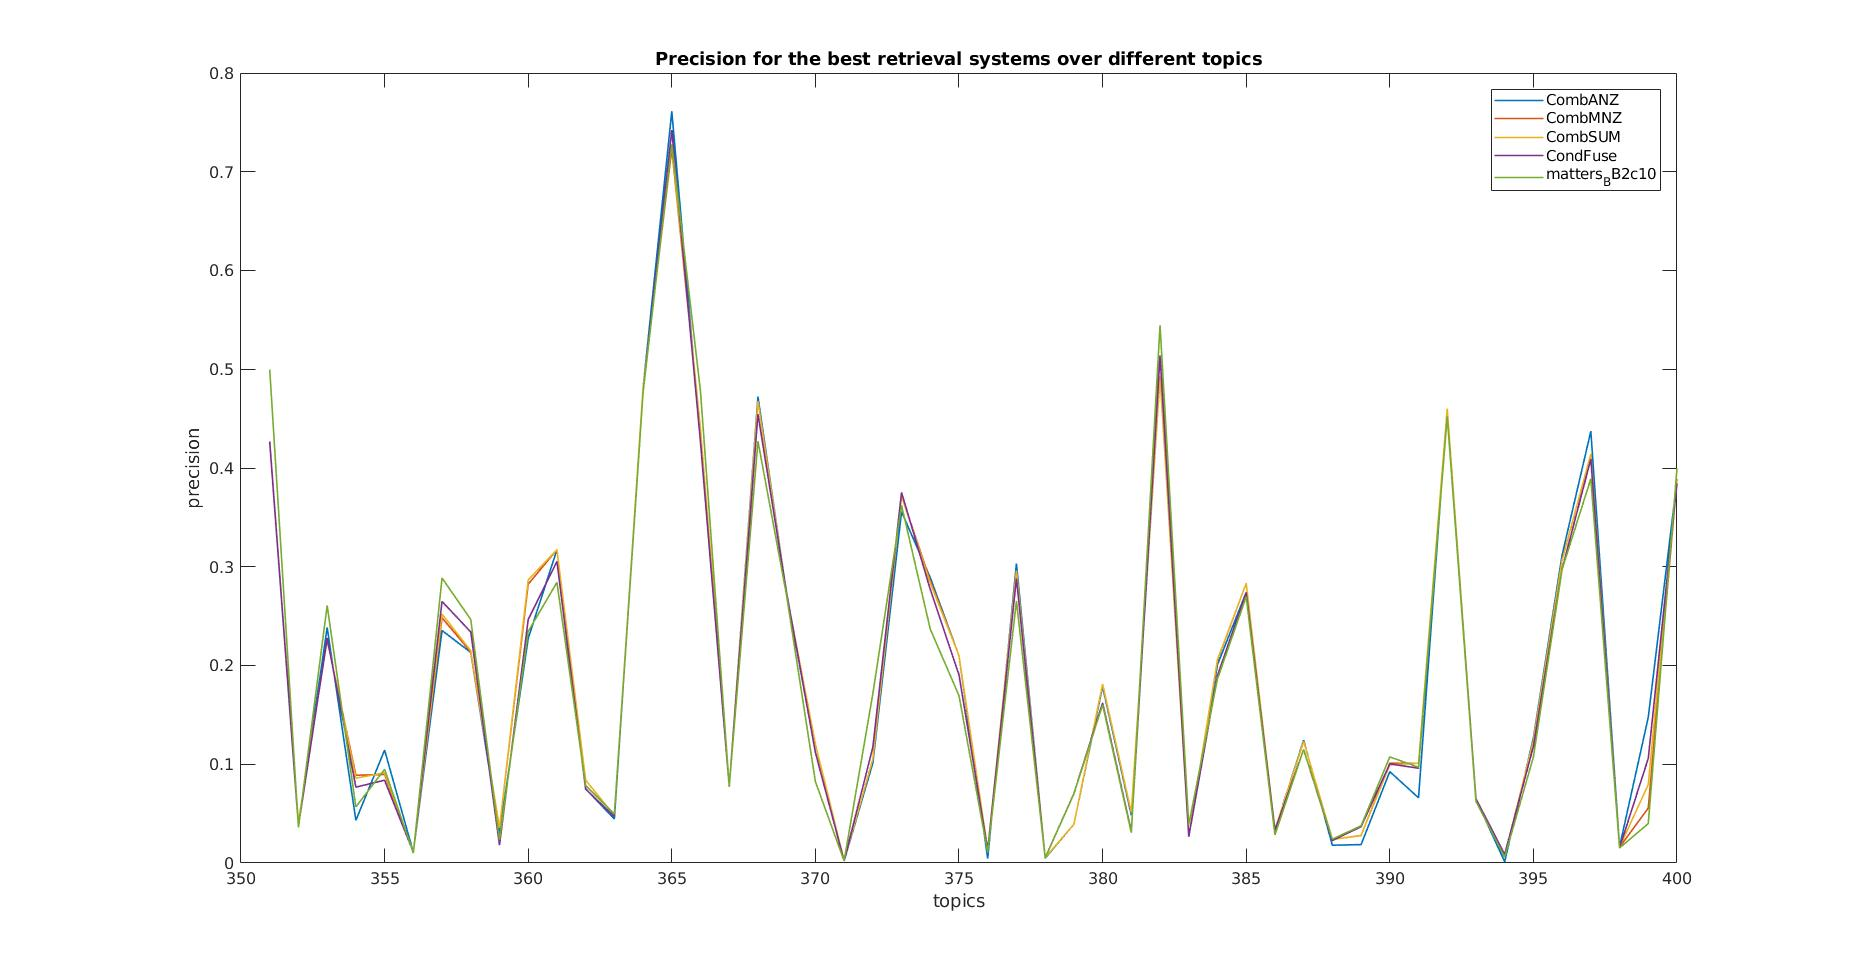
\includegraphics[width=\linewidth]{../eval/results-img-graphs/top5.jpg}
				\captionof{Figure 1: }{AP over 50 topics for the 5 best systems}				
				\label{fig:top5AP}					
			\end{minipage}
		\hfill	
			\begin{minipage}{0.3\linewidth}
				\begin{tabular}{c c}
					\toprule
					\textbf{Systems} & \textbf{MAP}\\ \toprule
					CombSUM & 0.1909 \\
					CombMNZ & 0.1902 \\
					CombANZ & 0.1891 \\
					CondFuse & 0.1883 \\
					BB2 & 0.1881 \\
					IFB2 & 0.1880 \\					
					DirichletLM & 0.1862 \\
					InL2 & 0.1853 \\
					CombMED & 0.1840 \\
					DLH13 & 0.1829 \\				
					BM25 & 0.1827 \\
					TF\_IDF & 0.1821\\
					CombMAX & 0.1817 \\
					DFIZ & 0.1783 \\					
					DFIC & 0.1758 \\				
					Hiemstra\_LM & 0.1733 \\
					CombMIN & 0.1515 \\							
					\bottomrule
				\end{tabular}
			\caption{Retrieval systems sorted by descreasing MAP}
			\label{tab:17SysMAP}
			\end{minipage}			
	\end{table}

	\subsubsection{Results Analysis}
	The results of these first tests show that it is generally convenient to use a fusion method.
	Four out of the top five best systems where fusion systems, with Condorcet Fuse beign the fourth best overall.
	
	But, we also noted that the performances of the methods are all very close, and the best and worse topics are the same regardless of the system used.

        \subsection{Evaluation metrics}
		% Perche abbiamo usato solo la MAP 
		% Perche' si fanno questi confronti

	    \subsection{Results}

		\begin{table}[H]
		    \centering
		    \begin{tabular}{c p{4cm}}
		    \toprule
		    \textbf{Fusion methods} & \textbf{MAP} \\ \toprule
		    CombMNZ &  \\ \hline
		    CombSUM &  \\ \hline
		    CombMIN &  \\ \hline
		    CombMAX &  \\ \hline
		    CombMED &  \\ \hline
		    CombANZ &  \\ \hline
			Condorcet &  \\ \bottomrule
		    \end{tabular}
		    \caption{Mean Average Precision for the 10 fused runs}
		\end{table}

	\section{Conclusions}
	
	\clearpage
	\begin{thebibliography}{1}
		\bibitem{1}Lee, Joon Ho. ``Combining multiple evidence from different properties of weighting schemes." Proceedings of the 18th annual international ACM SIGIR conference on Research and development in information retrieval. ACM, 1995.
		\bibitem{2}Fox, Edward A., and Joseph A. Shaw. ``Combination of multiple searches." NIST special publication SP 243 (1994).
		\bibitem{3}Montague, Mark, and Javed A. Aslam. ``Condorcet fusion for improved retrieval." Proceedings of the eleventh international conference on Information and knowledge management. ACM, 2002.
		
	\end{thebibliography}
	

\end{document}
